\usetikzlibrary{shapes.geometric}

\tikzset{elliparc/.style args={#1:#2:#3}{%
insert path={(#1:#3) arc (#1:#2:#3)}}}
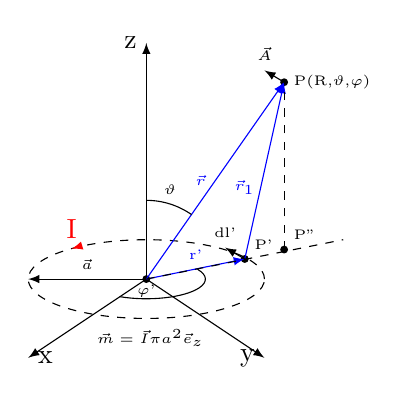
\begin{tikzpicture}

    %Elipse
    \node[ellipse,
        draw = black,
        dashed,
        minimum width = 3cm,
        minimum height = 1cm] (e) at (0,0) {};
    
    %Punkte
    \fill[](0,0)        circle(.05);
    \fill[](1.75,2.5)   circle(.05)
        node[right]{\tiny{P(R,$\vartheta$,$\varphi$)}};
    \fill[](1.25,0.255) circle(.05)
        node[above right]{\tiny{P'}};
    \fill[](1.75,0.375) circle(.05)
        node[above right]{\tiny{P''}};

    %Koordinaten Achsen
    \draw[-latex](0,0)--(-1.5,-1) node[right]{x};
    \draw[-latex](0,0)--(1.5,-1) node[left]{y};
    \draw[-latex](0,0)--(0,3) node[left]{z};
    
    %Pfeile
    \draw[-latex, blue](0,0)--(1.75,2.5)
        node[above, midway, left]{\tiny{$\vec{r}$}};
    \draw[-latex, blue](1.25,0.255)--(1.75,2.5)
        node[midway, below left]{\tiny{$\vec{r}_1$}};
    \draw[-latex, blue](0,0) -- (1.25,0.255)
        node[above, midway]{\tiny{\tiny{r}'}};
    \draw[-latex, red](-0.9,0.4)--(-.95,.385)
        node[above]{I};
    \draw[-latex](1.25,0.255)--(1,0.4)
        node[above]{\tiny{dl'}};
    \draw[-latex](1.75,2.5)--(1.5,2.65)
        node[above]{\tiny$\vec{A}$};
    \draw[-latex](0,0)--(-1.5,-0)
        node[above, midway]{\tiny$\vec{a}$};
   
    %Winkel
    \draw[-] (90:1) arc (90:55:1)
    node[above, midway] {\tiny{$\vartheta$}};
    \draw[] (0,0) [elliparc=-117:30:.75cm and .25cm];
    \node[yshift=-4.5]{\tiny{$\varphi$'}};
    
    %Legende
    \node[right] at (-0.75,-0.75){\tiny{$\vec{m}=\vec{I}\pi a^2\vec{e}_z$}};
   
    %Linien
    \draw[dashed](0,0)--(2.5,0.5);
    \draw[dashed](1.75,0.375)--(1.75,2.5);

\end{tikzpicture}
